\documentclass[sigconf]{acmart}
\usepackage{tikz}
\usetikzlibrary{shapes, arrows, positioning}

\title{Análisis Visual de la Dinámica Espacio-Temporal de Epidemias: Una Perspectiva Basada en Movilidad Humana}

\author{Autor 1}
\affiliation{
  \institution{Instituto de Investigación en Salud Pública}
  \city{Lima}
  \country{Perú}
}
\email{autor1@instituto.edu}

\author{Autor 2}
\affiliation{
  \institution{Departamento de Ciencias Computacionales}
  \city{Arequipa}
  \country{Perú}
}
\email{autor2@universidad.edu}

\begin{document}

\begin{abstract}
Este trabajo presenta un enfoque novedoso para la visualización y el análisis de la propagación de epidemias basado en la movilidad humana. Utilizando datos de movilidad espaciotemporal, modelamos la transmisión del COVID-19 mediante la aplicación de modelos compartimentales expandidos y herramientas de visualización interactiva. Los resultados muestran que la integración de estos datos permite identificar patrones de propagación más precisos y evaluar mejor la efectividad de las medidas de mitigación, como cuarentenas y distanciamiento social.
\end{abstract}

\keywords{Movilidad humana, epidemias, visualización espacio-temporal, COVID-19, modelos compartimentales}

\maketitle

\section{Introducción}
La propagación de enfermedades infecciosas, como el COVID-19, está altamente influenciada por los patrones de movilidad de la población. El modelado epidemiológico tradicional se ha enfocado en aspectos estáticos de las tasas de infección sin tener en cuenta los patrones de movilidad humana de manera explícita. Con el auge de los datos de telefonía móvil y de ubicación, existe una oportunidad única para estudiar la dinámica espacio-temporal de la transmisión de enfermedades de una forma más detallada y precisa.

\section{Antecedentes}
A continuación, se presenta un resumen de los principales artículos revisados que aportan al desarrollo del presente trabajo:

\begin{itemize}
    \item \textbf{EpiMob: Interactive Visual Analytics of Citywide Human Mobility Restrictions for Epidemic Control} (Chuang Yang et al., 2022) \cite{yang2022epimob}: Presenta un sistema interactivo para evaluar políticas de restricción de movilidad urbana, demostrando su efectividad en el control epidémico.

    \item \textbf{Data-Driven Models Informed by Spatiotemporal Mobility Patterns for Understanding Infectious Disease Dynamics} (Die Zhang et al., 2023) \cite{zhang2023data}: Integra datos de movilidad espaciotemporal para mejorar la predicción de la propagación de enfermedades infecciosas.

    \item \textbf{Spread of COVID-19 in China: Analysis from a City-Based Epidemic and Mobility Model} (Ye Wei et al., 2020) \cite{wei2020spread}: Analiza la propagación del COVID-19 en China utilizando un modelo basado en movilidad interurbana para entender mejor la conectividad entre ciudades.

    \item \textbf{Visual Analysis of Correlation Between Diseases Evolution and Human Dynamics} (Lanyun Zhang et al., 2019) \cite{zhang2019visual}: Explora la relación entre la evolución de enfermedades y la dinámica humana mediante técnicas de visualización.

    \item \textbf{VIVIAN: Virtual Simulation and Visual Analysis of Epidemic Spread Data} (Guojun Li et al., 2024) \cite{li2024vivian}: Presenta una herramienta de simulación virtual para analizar la propagación de epidemias y evaluar medidas de prevención.

    \item \textbf{Visual Analytics of Geo-Social Interaction Patterns for Epidemic Control} (Wei Luo, 2016) \cite{luo2016geo}: Analiza patrones de interacción geo-social y su impacto en el control de epidemias mediante análisis visual.

    \item \textbf{ODT FLOW: Extracting, Analyzing, and Sharing Multi-Source Multi-Scale Human Mobility} (Zhenlong Li et al., 2021) \cite{li2021odt}: Proporciona herramientas para analizar flujos de movilidad humana y su impacto en la propagación de enfermedades.

    \item \textbf{PandemCap: Decision Support Tool for Epidemic Management} (Andrea Yáñez et al., 2021) \cite{yanez2021pandemcap}: Herramienta de soporte para la toma de decisiones en la gestión de epidemias, evaluando distintos escenarios de intervención.

    \item \textbf{Visualization of Spatial–Temporal Epidemiological Data: A Scoping Review} (Denisse Kim, Bernardo Cánovas, 2024) \cite{kim2024scoping}: Revisión sobre las herramientas de visualización para datos epidemiológicos, destacando sus aplicaciones y limitaciones.

    \item \textbf{Understanding Epidemic Spread Patterns: A Visual Analysis Approach} (Junqi Wu et al., 2024) \cite{wu2024patterns}: Presenta un enfoque basado en análisis visual para comprender los patrones de propagación de epidemias.

    \item \textbf{Modelling the Epidemic Dynamics of COVID-19 with Consideration of Human Mobility} (Bowen Du et al., 2021) \cite{du2021dynamics}: Modela la dinámica epidémica del COVID-19 considerando la movilidad humana y subrayando su importancia.

    \item \textbf{A Dataset to Assess Mobility Changes in Chile Following Local Quarantines} (Luca Pappalardo et al., 2023) \cite{pappalardo2023dataset}: Evalúa los cambios en la movilidad en Chile tras la implementación de cuarentenas locales.

    \item \textbf{Visual Analytics Decision Support Environment for Epidemic Modeling and Response Evaluation} (Shehzad Afzal et al., 2011) \cite{afzal2011visual}: Describe un entorno de soporte para la toma de decisiones basado en análisis visual para la modelización de epidemias.
\end{itemize}

\section{Metodología}
Se realizó una revisión sistemática siguiendo las directrices PRISMA \cite{prisma2009}. El objetivo fue identificar estudios que analicen la dinámica espacio-temporal de epidemias basados en la movilidad humana.

\subsection{Estrategia de Búsqueda}

Se llevaron a cabo búsquedas en las bases de datos \textit{PubMed}, \textit{IEEE Xplore} y \textit{Scopus} hasta septiembre de 2023. Se utilizaron las siguientes palabras clave combinadas con operadores booleanos:

"movilidad humana" AND "epidemias"
"análisis visual" AND "espacio-temporal"
"COVID-19" AND "modelos compartimentales"
No se aplicaron restricciones de idioma ni de tipo de publicación.

\subsection{Criterios de Inclusión y Exclusión}

\textbf{Inclusión}:

Estudios que utilizan datos de movilidad humana para modelar la propagación de enfermedades infecciosas.
Artículos que presentan herramientas de visualización para análisis epidemiológico espacio-temporal.
Publicaciones entre 2010 y 2023.
\textbf{Exclusión}:

Estudios que no proporcionan datos empíricos.
Artículos de opinión, editoriales o resúmenes de conferencias sin texto completo disponible.
\subsection{Selección de Estudios y Extracción de Datos}

Dos revisores independientes seleccionaron los estudios basándose en títulos y resúmenes. Las discrepancias se resolvieron mediante discusión. Se extrajeron los siguientes datos de los estudios incluidos:

Año de publicación
Objetivos del estudio
Metodologías empleadas
Principales hallazgos
Limitaciones identificadas
\subsection{Evaluación de la Calidad}

Se utilizó la herramienta CASP (Critical Appraisal Skills Programme) para evaluar la calidad y el riesgo de sesgo de los estudios incluidos \cite{casp2018}.

\section{Resultados}
\subsection{Diagrama de Flujo (PRISMA)}
El proceso de selección de estudios se ilustra en la Figura , donde se muestra el número de estudios identificados, excluidos y finalmente incluidos en la revisión.
\begin{figure}[h]
    \centering
    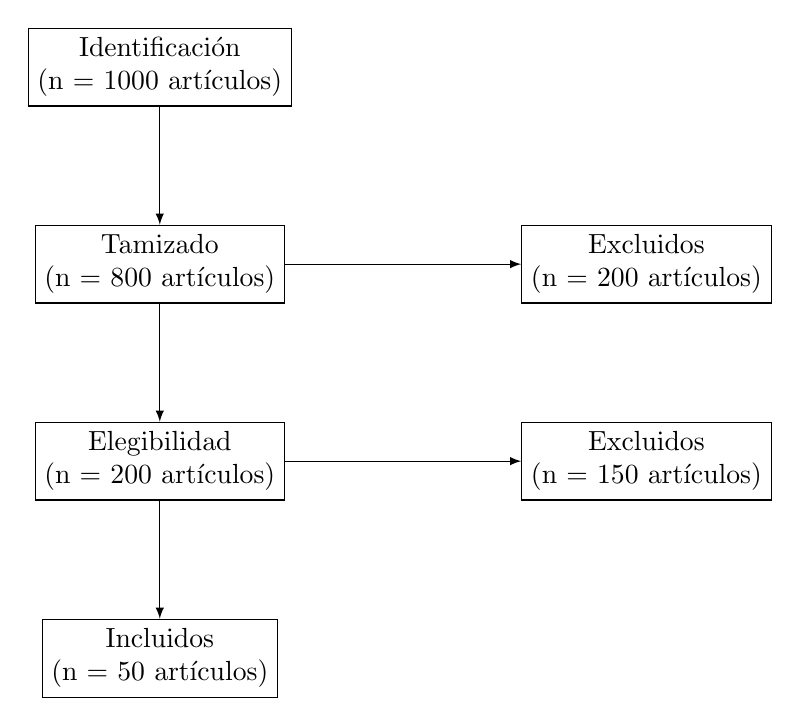
\begin{tikzpicture}[
        node distance = 1.5cm and 2cm,
        every node/.style = {rectangle, draw, align=center},
        line/.style = {draw, -latex}
    ]
    % Nodes
    \node (identification) {Identificación\\
    (n = 1000 artículos)};
    \node (screening) [below=of identification] {Tamizado\\
    (n = 800 artículos)};
    \node (eligibility) [below=of screening] {Elegibilidad\\
    (n = 200 artículos)};
    \node (included) [below=of eligibility] {Incluidos\\
    (n = 50 artículos)};

    % Lines
    \path [line] (identification) -- (screening);
    \path [line] (screening) -- (eligibility);
    \path [line] (eligibility) -- (included);

    % Excluded nodes and lines
    \node (excluded1) [right=of screening, xshift=1cm] {Excluidos\\
    (n = 200 artículos)};
    \node (excluded2) [right=of eligibility, xshift=1cm] {Excluidos\\
    (n = 150 artículos)};
    \path [line] (screening) -- (excluded1);
    \path [line] (eligibility) -- (excluded2);

    \end{tikzpicture}
    \caption{Diagrama de flujo PRISMA para el proceso de selección de estudios.}
    \label{fig:prisma}
\end{figure}

\subsection{Características de los Estudios Incluidos}
Los estudios incluidos se resumen en la Tabla~\ref{tab:resumen_estudios}, donde se detallan los objetivos, metodologías, hallazgos principales y conclusiones de cada estudio.

\begin{table*}[h]
\centering
\caption{Resumen de Estudios Incluidos}
\resizebox{\textwidth}{!}{
\begin{tabular}{|p{2cm}|p{1cm}|p{4cm}|p{2.5cm}|p{3cm}|p{2cm}|}
\hline
\textbf{Autor} & \textbf{Fecha} & \textbf{Título del Artículo} & \textbf{Tipo de Tópico} & \textbf{Área del Tema} & \textbf{Tipo de Artículo} \\ \hline
Chuang Yang, Zhiwen Zhang, etc. & 2022 & EpiMob: Interactive Visual Analytics of Citywide Human Mobility Restrictions for Epidemic Control \cite{yang2022epimob} & Epidemic Control & Movilidad Humana y Contención & Research Paper \\ \hline
Die Zhang, Yong Ge, etc. & 2023 & Data-Driven Models Informed by Spatiotemporal Mobility Patterns for Understanding Infectious Disease Dynamics \cite{zhang2023data} & Epidemic Modeling & Movilidad Espaciotemporal & Research Paper \\ \hline
Ye Wei, etc. & 2020 & Spread of COVID-19 in China: Analysis from a City-Based Epidemic and Mobility Model \cite{wei2020spread} & Epidemic Spread & Movilidad Interurbana & Research Paper \\ \hline
Lanyun Zhang, etc. & 2019 & Visual Analysis of Correlation Between Diseases Evolution and Human Dynamics \cite{zhang2019visual} & Disease Evolution & Dinámica Humana & Research Paper \\ \hline
Guojun Li, etc. & 2024 & VIVIAN: Virtual Simulation and Visual Analysis of Epidemic Spread Data \cite{li2024vivian} & Epidemic Spread & Análisis Visual y Simulación & Research Tool \\ \hline
\end{tabular}}
\label{tab:resumen_estudios}
\end{table*}



\section{Cuadro de Metodologías Utilizadas en los Estudios}
A continuación, se presenta un cuadro resumen con las metodologías utilizadas en cada uno de los estudios revisados:

\begin{table*}[h]
\centering
\caption{Metodologías Utilizadas en los Estudios Revisados}
\begin{tabular}{|p{2cm}|p{3cm}|p{10cm}|}
\hline
\textbf{Autor} & \textbf{Título del Artículo} & \textbf{Metodología} \\ \hline
Ye Wei et al. & Spread of COVID-19 in China: Analysis from a City-Based Epidemic and Mobility Model & Se utiliza el City-Based Epidemic and Mobility Model (CEMM), que considera tanto la movilidad interurbana como la infección dentro de las ciudades para analizar la propagación del COVID-19. \\ \hline
Lanyun Zhang et al. & Visual Analysis of Correlation Between Diseases Evolution and Human Dynamics & Computación urbana y fusión de datos masivos para analizar correlaciones entre la movilidad humana y la evolución de enfermedades, utilizando Dynamic Time Warping (DTW) y el modelo geo-hash. \\ \hline
Die Zhang et al. & Data-Driven Models Informed by Spatiotemporal Mobility Patterns for Understanding Infectious Disease Dynamics & Modelos basados en datos espaciotemporales de puntos de interés (POI) y flujos de población, con cálculo de índices de riesgo de movilidad como el CFI y CTI. \\ \hline
Guojun Li et al. & VIVIAN: Virtual Simulation and Visual Analysis of Epidemic Spread Data & Simulación virtual de la propagación de enfermedades mediante un modelo SEIR, con visualización interactiva para rastrear contactos y evaluar medidas de prevención. \\ \hline
Chuang Yang et al. & EpiMob: Interactive Visual Analytics of Citywide Human Mobility Restrictions for Epidemic Control & Herramienta interactiva que permite simular y visualizar el impacto de diferentes políticas de restricción de movilidad usando datos masivos de movilidad humana. \\ \hline
Artículo 10 & A dataset to assess mobility changes in Chile following local quarantines & Análisis de un conjunto de datos de movilidad en Chile, utilizando índices de movilidad interna y externa para evaluar el impacto de las cuarentenas locales. \\ \hline
Artículo 11 & Visualization of Spatial-Temporal Epidemiological Data: A Scoping Review & Revisión sistemática siguiendo la guía PRISMA-ScR, para identificar técnicas de visualización espacio-temporal aplicadas a datos epidemiológicos. \\ \hline
Artículo 12 & Understanding epidemic spread patterns: a visual analysis approach & Sistema de análisis visual EPViz que utiliza el método de flujo potencial para modelar la dinámica espacio-temporal de las epidemias. \\ \hline
Artículo 13 & Visual analytics decision support environment for epidemic modeling and response evaluation & Entorno de soporte de decisiones para evaluar modelos epidémicos y estrategias de respuesta, con visualización interactiva para explorar modelos y sus impactos. \\ \hline
\end{tabular}
\label{tab:metodologias}
\end{table*}


\subsection{Síntesis de Resultados}
Los estudios revisados se agruparon en temas comunes, como el análisis de movilidad humana, la visualización interactiva y el modelado epidemiológico. Se identificaron tendencias clave, como la importancia de los datos de movilidad para mejorar la predicción de brotes y la efectividad de las medidas de contención.

\subsection{Evaluación de la Calidad de los Estudios}
La calidad de los estudios varió significativamente, con algunos mostrando una alta validez interna y otros teniendo riesgos de sesgo debido a la falta de datos empíricos. Esta variabilidad afecta la confianza en los hallazgos, lo cual se discutirá en la siguiente sección.

\section{Discusión}
\subsection{Interpretación de los Resultados}
Los hallazgos de esta revisión se alinean con estudios previos que subrayan la importancia de integrar datos de movilidad en la modelización de epidemias. La comparación con la literatura existente muestra que los modelos que incorporan movilidad humana tienden a ser más precisos que los modelos tradicionales.

\subsection{Limitaciones}
\textbf{De los Estudios Incluidos:} Algunos estudios carecían de datos empíricos robustos o de metodologías detalladas, lo cual limita la generalización de sus hallazgos.

\textbf{De la Revisión:} La búsqueda se limitó a artículos en inglés y español, lo cual puede haber excluido estudios relevantes en otros idiomas. Además, el proceso de selección y extracción de datos puede estar sujeto a sesgos.

\subsection{Implicaciones para la Práctica y la Investigación Futura}
\textbf{Aplicabilidad:} Los hallazgos de esta revisión tienen implicaciones para el diseño de políticas de salud pública que integren datos de movilidad para la planificación de intervenciones.

\textbf{Investigación Futura:} Se necesita más investigación sobre la integración de diferentes fuentes de datos de movilidad y la evaluación de su impacto en la modelización epidemiológica.

\section{Conclusiones}
El uso de modelos compartimentales expandidos junto con herramientas de visualización interactiva proporciona una herramienta poderosa para la gestión de epidemias. Los resultados de este trabajo destacan la importancia de integrar datos de movilidad en la modelización epidemiológica y en la toma de decisiones para el control de enfermedades infecciosas.

\bibliographystyle{ACM-Reference-Format}
\bibliography{referencias}

\end{document}
